\documentclass[a4paper]{article}

\usepackage[T1]{fontenc}
\usepackage{graphicx}
\usepackage{amsmath}
\usepackage[utf8]{inputenc}
\usepackage{enumitem}
\setlist[description]{style=unboxed}

\usepackage{tikz}
\usepackage{pgfplots}
\usepackage{circuitikz}
\usepackage{tabularx}
\usepackage{rotating}

\usetikzlibrary{calc,positioning,shapes,decorations.pathreplacing}

\tikzset{
	short/.style={draw,rectangle,text height=3pt,text depth=13pt,
		text width=7pt,align=center,fill=gray!30},
	long/.style={short,text width=1.5cm},
	verylong/.style={short,text width=4.5cm}
}

\begin{document}
\section{AC voltage rectifier and regulator}

\subsection{Introduction}

For fully functional operation, submarine/robot arm/habitat is equipped with 
lot of computer based subsystems and electronic devices which operate on DC 
voltage. To ensure proper operation the DC voltage has to be stable and without 
noise. To ensure stable DC voltage, linear regulator on Fig. 1. is used. Due to 
extreme conditions in the system, regulators often fail and components have to 
be repaired or replaced with proper spare part.

In this task, your job is to:
\begin{itemize}
\item find the parts which ensure proper operation of regulator, 
\item ensure that the output voltage ripple is within the boundaries with 
proper low pass filter,
\item find the probability of future malfunction in standby redundant system.
\end{itemize}

\textbf{Regulator specifications.} Regulator specifications are provided with 
the following table. In each task you have to ensure that the values specified
in the table correspond to the values which will be measured in simulation. 

\begin{table}[h!]
    \hyphenpenalty 10000
    \caption{Regulator specifications}
    \label{tab:spec}
    \begin{tabularx}{\linewidth}{|X|X|X|X|} \hline
    PARAMETER & TEST CONDITIONS & VALUE & UNIT \\ \hline 
    Output voltage ($V_o$)& $I_o = 1$ A & $10.00$ & V \\ \hline
    Output current ($I_o$) & a & $1.5$ & A \\ \hline
    Ripple rejection & (50 Hz) & $78$ & dB \\ \hline
   	Dropout voltage & $I_o = 1.5$ A & $2$ & V \\ \hline
    \end{tabularx}
\end{table}

\newpage

\subsection{Finding the proper choice of components}
\label{ele:task:1}
As it can be seen in regulator scheme, some components are not determined. In 
this subtask you need to specify resistor $R_1$ and diode $D_1$. Additionally, 
you have to determine positions of the negative and the positive input of the 
amplifier $A_1$. Based on the regulators operating values provided with table
\ref{tab:spec} and regulator test points diagrams (Fig. 1. - Fig. 5) you have 
to determine specifications for the resistor $R_1$ and diode $D_1$. You have to 
find the real components from the DigiKey Electronics product database. 

There are, however, constraints for your choice of components:
\begin{itemize}
\item $R_1$ has footprint given with figure Fig. \ref{fig:footprint},
\item $D_1$ is a through-hole component.
\end{itemize} 
 
Your choice is graded in several ways:
\begin{itemize}
\item component price,
\item correct component voltage, power and current ratings,
\item correct component footprint.
\end{itemize}
As a result, you have to provide two DigiKey part numbers for resistor and 
diode, respectively. 

\subsection{LC filter design}
\label{ele:task:2}
To achieve specified ripple rejection at required frequency, design a LC low 
pass filter which filters output of a regulator. As in previous task you have 
to provide DigiKey part numbers for LC filter. 

Again, there are constraints for your choice of components:
\begin{itemize}
\item $L_1$ has nameof footprint,
\item $C_2$ has to be a ceramic capacitor with footprint given with 
\ref{fig:footprint2}. 
\end{itemize}

Your choice is graded in the similar fashion as before:
\begin{itemize}
\item price,
\item correct inductance and capacitance,
\item correct footprints, 
\item correct current and voltage ratings.
\end{itemize}
As a result, you have to provide two DigiKey part numbers for inductor and 
capacitor, respectively. 

\subsection{Side task: Reliability of redundant linear regulator system}
\label{ele:task:3}
To increase reliability of the power supply system two different linear 
regulators are linked in configuration which is given with the Fig. 
\ref{fig:psc}. This configuration is known as passive standby redundancy. 
Probability of a failure in one regulator is modeled with exponential 
probability density function. More precisely, probability density function for 
the first regulator is:  
\begin{equation}
f_1(t) = \lambda_1 e^{-\lambda_1 t}
\end{equation}
and for the second regulator:
\begin{equation}
f_2(t) = \lambda_2 e^{-\lambda_2 t}
\end{equation}

Your task is to determine probability density function $f_S(t)$ which gives the
probability of failure in system described with Fig. \ref{fig:psc}. As a result 
provide probability of a failure for $t = 1000$ $h$ with:
\begin{itemize}
\item[] $\lambda_1 = 1 \cdot10^{-6}$ $h^{-1}$
\item[] $\lambda_2 = 2 \cdot10^{-6}$ $h^{-1}$ 
\end{itemize} 

\textbf{Note}: time to failure is increased $T_{fs} = T_{1f} + T_{2f}$. 

\subsection{Solution format}
Solution for each task is a plain text document containing requested data. For
the tasks \ref{ele:task:1} and \ref{ele:task:2} text documents need to have 
two rows. One component part number in each row. Only one row is needed for the 
task \ref{ele:task:3} (requested probability). Name the files 
\texttt{task1.txt}, \texttt{task2.txt}, \texttt{task3.txt} and put them in 
the appropriate Google Drive folder.

Additionally, for the task \ref{ele:task:3} you have to provide documentation.

\subsection{Grading scheme}
Tasks are graded in the following manner:
\begin{itemize}
\item tasks \ref{ele:task:1} and \ref{ele:task:2} - up to \textbf{10 pts}, 
up to \textbf{5 pts} for each component.
\item task \ref{ele:task:3} - up to \textbf{10 pts} - \textbf{5 pts} for the 
correct probability and up to \textbf{5 pts} for correct documentation.
\end{itemize}



\begin{sidewaysfigure}[h!]
\centering
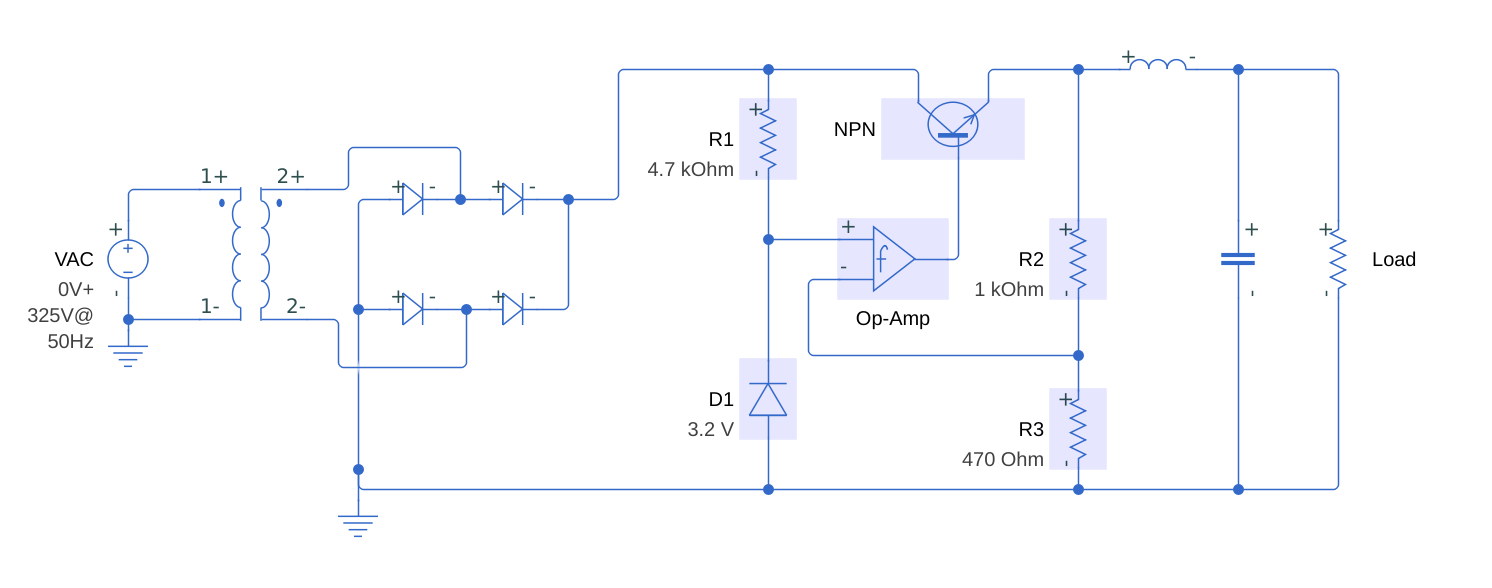
\includegraphics[width=\linewidth]{images/reg.png}
\caption{Rectifier and linear regulator.}
\end{sidewaysfigure}


 
\end{document}